\documentclass[%
 reprint,
%superscriptaddress,
%groupedaddress,
%unsortedaddress,
%runinaddress,
%frontmatterverbose, 
%preprint,
%preprintnumbers,
%nofootinbib,
%nobibnotes,
%bibnotes,
 amsmath,amssymb,
 aps,
%pra,
%prb,
%rmp,
%prstab,
%prstper,
%floatfix,
]{revtex4-2}

\usepackage{graphicx}
\usepackage{dcolumn}
\usepackage{bm}
\usepackage{tabularx}
\usepackage[utf8]{inputenc}
\usepackage[T1]{fontenc}
\usepackage{listings}
\usepackage{algpseudocode}
\usepackage[breaklinks, hidelinks, colorlinks=true,linkcolor=blue,citecolor=blue]
{hyperref}

\begin{document}

\title{Variação de Hiperparâmetros do Decodificador em Segmentação de Imagens}

\author{Wesley Nogueira Galvão}
\affiliation{Universidade Federal de São Carlos}

\date{\today}

\begin{abstract}
Este relatório apresenta uma investigação sobre o impacto da variação dos hiperparâmetros do decodificador na arquitetura EncoderDecoder para segmentação de imagens, utilizando o dataset Oxford-IIIT Pet. Foram avaliadas diferentes configurações de strides e a inclusão de camadas extras no decodificador, analisando o desempenho de segmentação e o custo computacional de cada modelo.
\end{abstract}

\maketitle

\section{Introdução}
A segmentação de imagens representa uma tarefa fundamental em Visão Computacional, com aplicações em áreas como medicina, agricultura, veículos autônomos e robótica. O avanço das redes neurais convolucionais (CNNs) proporcionou melhorias significativas de desempenho, especialmente com arquiteturas EncoderDecoder, que combinam extração de atributos e reconstrução espacial para gerar máscaras de segmentação precisas.

\subsection{Motivação}
Decodificadores flexíveis possibilitam a adaptação da arquitetura para diferentes níveis de detalhe e custo computacional. A escolha dos strides e a inclusão de camadas extras impactam diretamente a capacidade do modelo de recuperar detalhes espaciais e a eficiência do treinamento. Métodos como o EncoderDecoder são especialmente relevantes em cenários nos quais a precisão da segmentação é crítica, como na detecção de tumores ou segmentação de objetos em ambientes complexos.

\section{Objetivos}
\begin{enumerate}
    \item Avaliar o impacto da variação dos hiperparâmetros do decodificador na qualidade da segmentação.
    \item Comparar o custo computacional das diferentes configurações.
    \item Discutir vantagens e limitações de cada abordagem.
\end{enumerate}

\section{Metodologia}
\subsection{Conjunto de Dados}

O Oxford-IIIT Pet Dataset, ilustrado na Figura \ref{fig:image_gt_grid}, foi utilizado, e é composto por 7349 imagens de animais de estimação e suas respectivas máscaras de segmentação. O conjunto de teste contém 3669 imagens, enquanto 3680 imagens foram separadas para treino e validação (80\% para treino e 20\% para validação), com embaralhamento e semente fixa para garantir reprodutibilidade. Todas as imagens possuem anotações trimap, com pixels classificados como 1: região do animal (foreground), 2: fundo (background) e 3: não classificados (pixels ignorados).

\begin{figure*}[htb]
    \centering
    \label{fig:image_gt_grid}  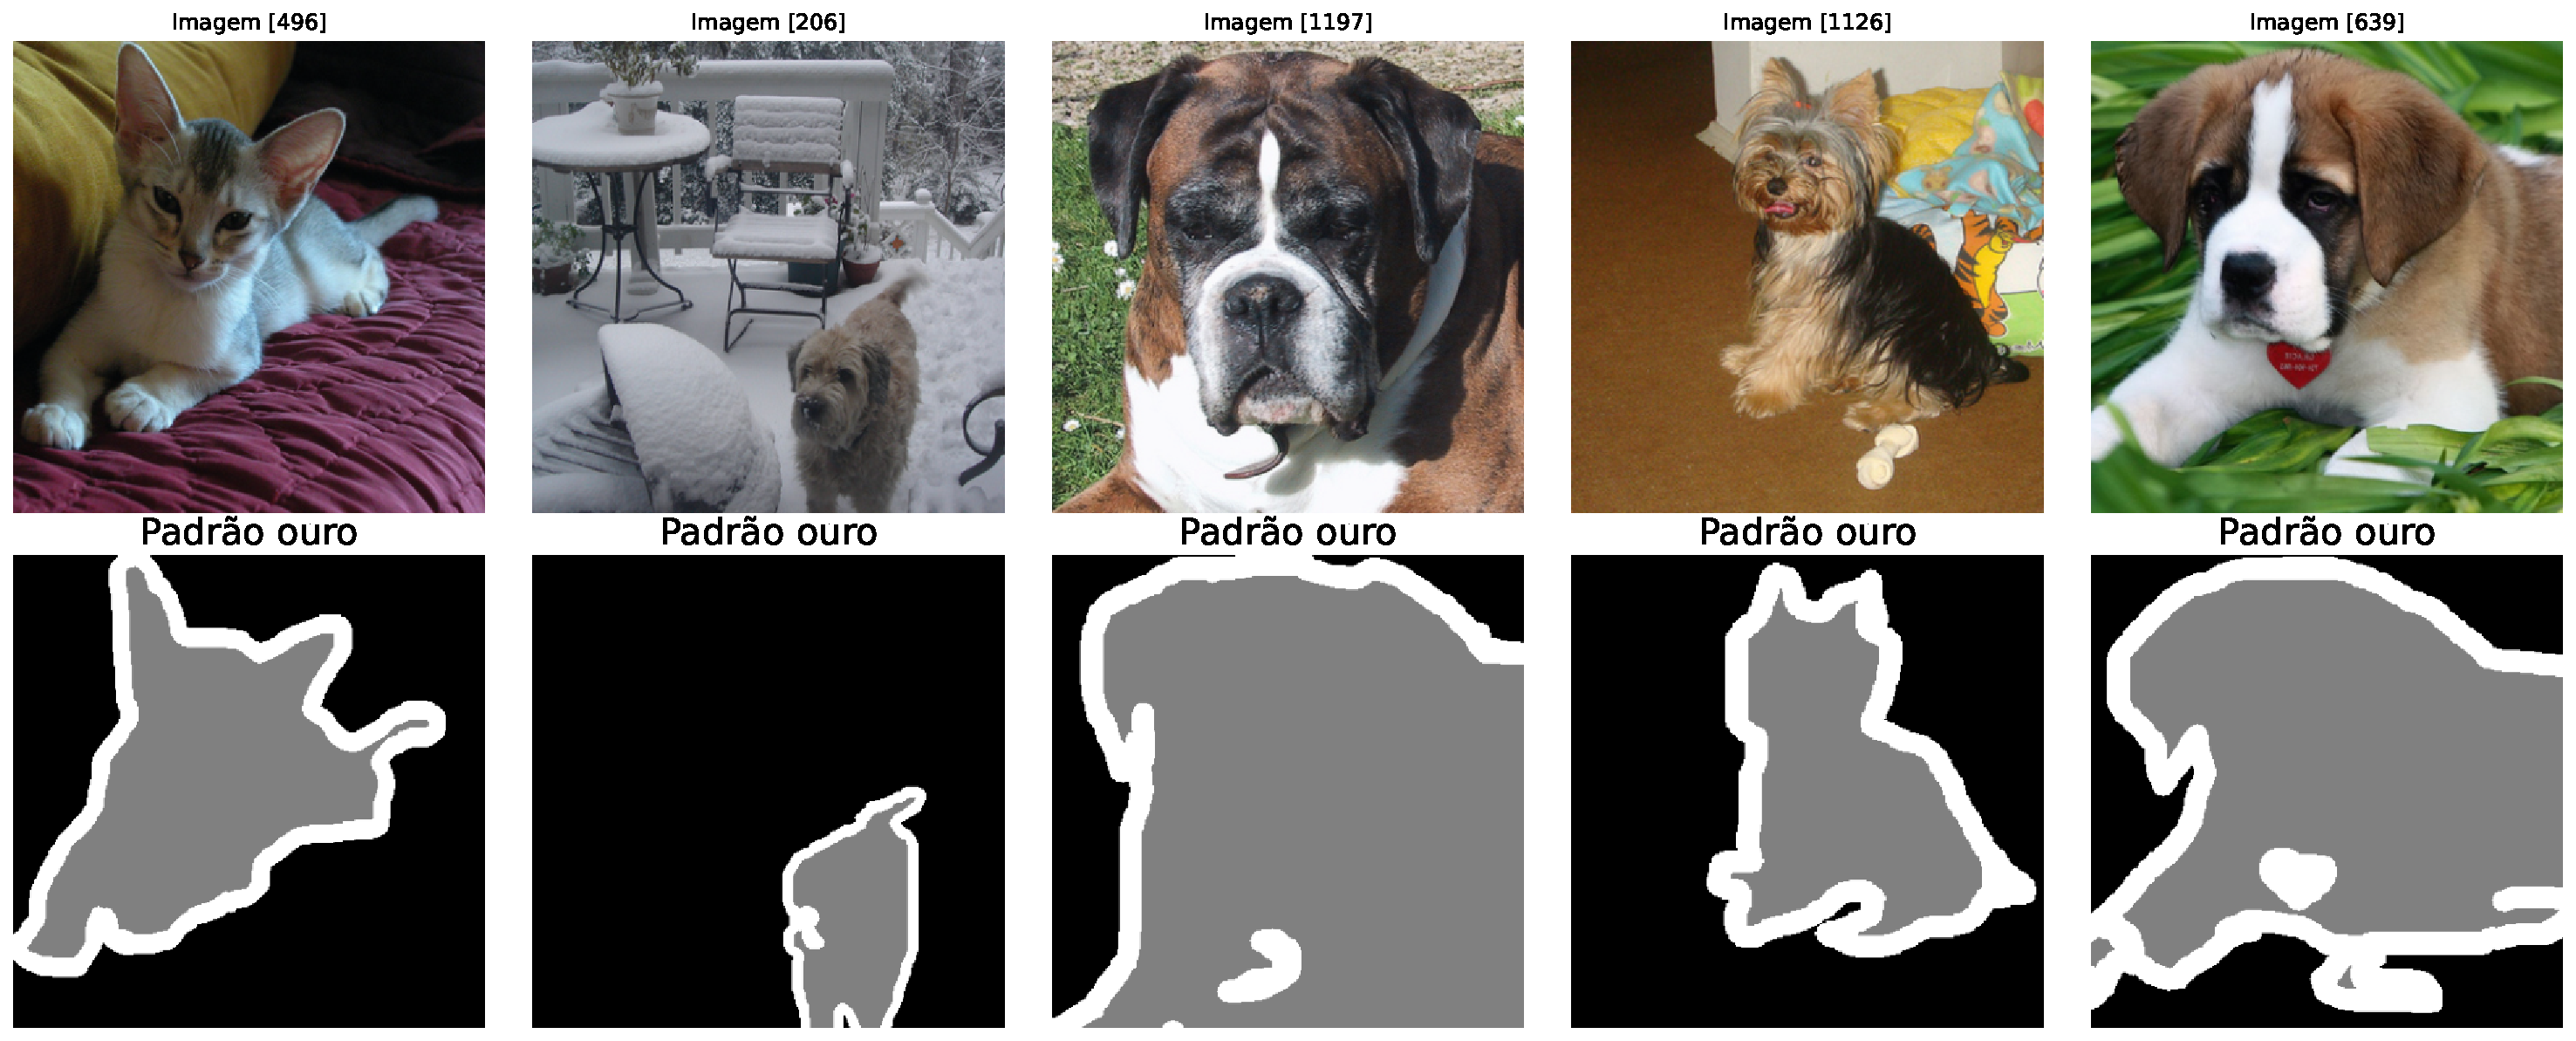
\includegraphics[width=0.98\textwidth]{imgs/image_gt_grid.pdf}
    \caption{Exemplo de imagens do conjunto de dados e suas respectivas máscaras de segmentação. As máscaras possuem três classes: fundo, região do animal e região de pixels a serem ignorados.}
\end{figure*}

\subsection{Arquitetura EncoderDecoder}
A arquitetura EncoderDecoder consiste em um encoder ResNet50 pré-treinado no ImageNet, responsável pela extração de atributos em diferentes resoluções (strides 2, 4, 8, 16, 32), e um decodificador que reconstrói a máscara de segmentação a partir desses atributos. O decodificador pode ser configurado para utilizar diferentes combinações de strides e incluir camadas extras de convolução, batch normalization e ReLU.

\subsection{Variações do Decodificador}
As seguintes configurações foram avaliadas:
\begin{itemize}
    \item Utilizar apenas os atributos no stride 32
    \item Utilizar apenas os atributos no stride 2
    \item Utilizar os atributos nos strides 2 e 32
    \item Utilizar os atributos nos strides 2, 8 e 32
    \item Utilizar os atributos nos strides 2 e 32 com camadas conv-batchnorm-relu extras em cada bloco do decodificador
\end{itemize}

\subsection{Procedimento Experimental}
Cada modelo foi treinado por 10 épocas, utilizando o encoder pré-treinado, batch size 128 para treino e 16 para validação, learning rate $1\times10^{-2}$ e weight decay $1\times10^{-3}$. O desempenho foi avaliado pela métrica de IoU (Intersecção sobre a União) e pelo tempo total de inferência.

\subsection{Teoria do Método}

O EncoderDecoder combina extração de atributos em múltiplas escalas com reconstrução espacial. O encoder gera tensores de diferentes resoluções, que são combinados pelo decodificador para recuperar detalhes espaciais. A escolha dos strides define o nível de detalhe e o custo computacional. A inclusão de camadas extras no decodificador pode aumentar a capacidade de modelagem, mas também o custo computacional.

O processo de segmentação inicia-se pela extração das ativações intermediárias do encoder ResNet, realizadas pela função \texttt{get\_features}. Essa função percorre as principais camadas do encoder, coletando tensores em diferentes resoluções (strides), que são utilizados pelo decodificador para reconstruir a máscara de segmentação.

Essas features correspondem aos mapas de ativação em múltiplas escalas, permitindo ao decodificador combinar detalhes locais e contexto global. O pseudocódigo abaixo ilustra esse processo.

\begin{algorithmic}[1]
\State \textbf{Input:} Imagem de entrada $x$
\State $x \gets$ conv1($x$)
\State $x \gets$ bn1($x$)
\State $x \gets$ relu($x$)
\State features.append($x$)
\State $x \gets$ maxpool($x$)
\For{cada bloco do encoder (layer1 a layer4)}
    \State $x \gets$ bloco($x$)
    \State features.append($x$)
\EndFor
\State \textbf{Output:} Lista de features em diferentes resoluções
\end{algorithmic}

No fluxo completo, as features extraídas por \texttt{get\_features} alimentam o decodificador, que as processa conforme o pseudocódigo anterior, combinando-as para gerar a máscara segmentada final.

\begin{algorithmic}[1]
\State \textbf{Input:} Lista de tensores de atributos $features$, lista de strides $S$, número de canais $C$, flag $extra\_convs$
\State Inverter ordem dos $features$ e $S$
\State $x \gets$ camada convolucional inicial em $features[0]$
\For{$i = 1$ até $|features|-1$}
    \State $x \gets$ interpolar $x$ para resolução de $features[i]$
    \State $x \gets$ $x$ + ajuste de canais de $features[i]$
    \If{$extra\_convs$}
        \State $x \gets$ conv-batchnorm-relu extra
    \EndIf
\EndFor
\State $mask \gets$ camada de classificação em $x$
\State \textbf{Output:} $mask$
\end{algorithmic}

O parâmetro \texttt{extra\_convs} permite adicionar uma camada extra de convolução, normalização e ativação (conv-batchnorm-relu) em cada bloco do decodificador. Essa camada adicional aumenta a capacidade de modelagem do decodificador, tornando-o capaz de capturar padrões mais complexos e refinar a reconstrução espacial das máscaras de segmentação.


\section{Resultados}


\subsection{Métricas de Treinamento}

Na Figura~\ref{fig:training_metrics}, é possível observar o comportamento das curvas de \textit{train\_loss}, \textit{valid\_loss} e \textit{IoU} para cada arquitetura de decodificador avaliada. Os modelos de alto desempenho — strides\_2\_8\_32, strides\_2\_32, strides\_2\_32\_extra\_convs e strides\_32 — apresentam curvas de perda decrescentes e suaves ao longo das épocas, o que indica um processo de treinamento estável e eficaz. As curvas de validação acompanham de perto as de treino, sem sinais evidentes de overfitting, reforçando a capacidade de generalização desses modelos.

\begin{figure*}[htb]
    \centering
    \label{fig:training_metrics}  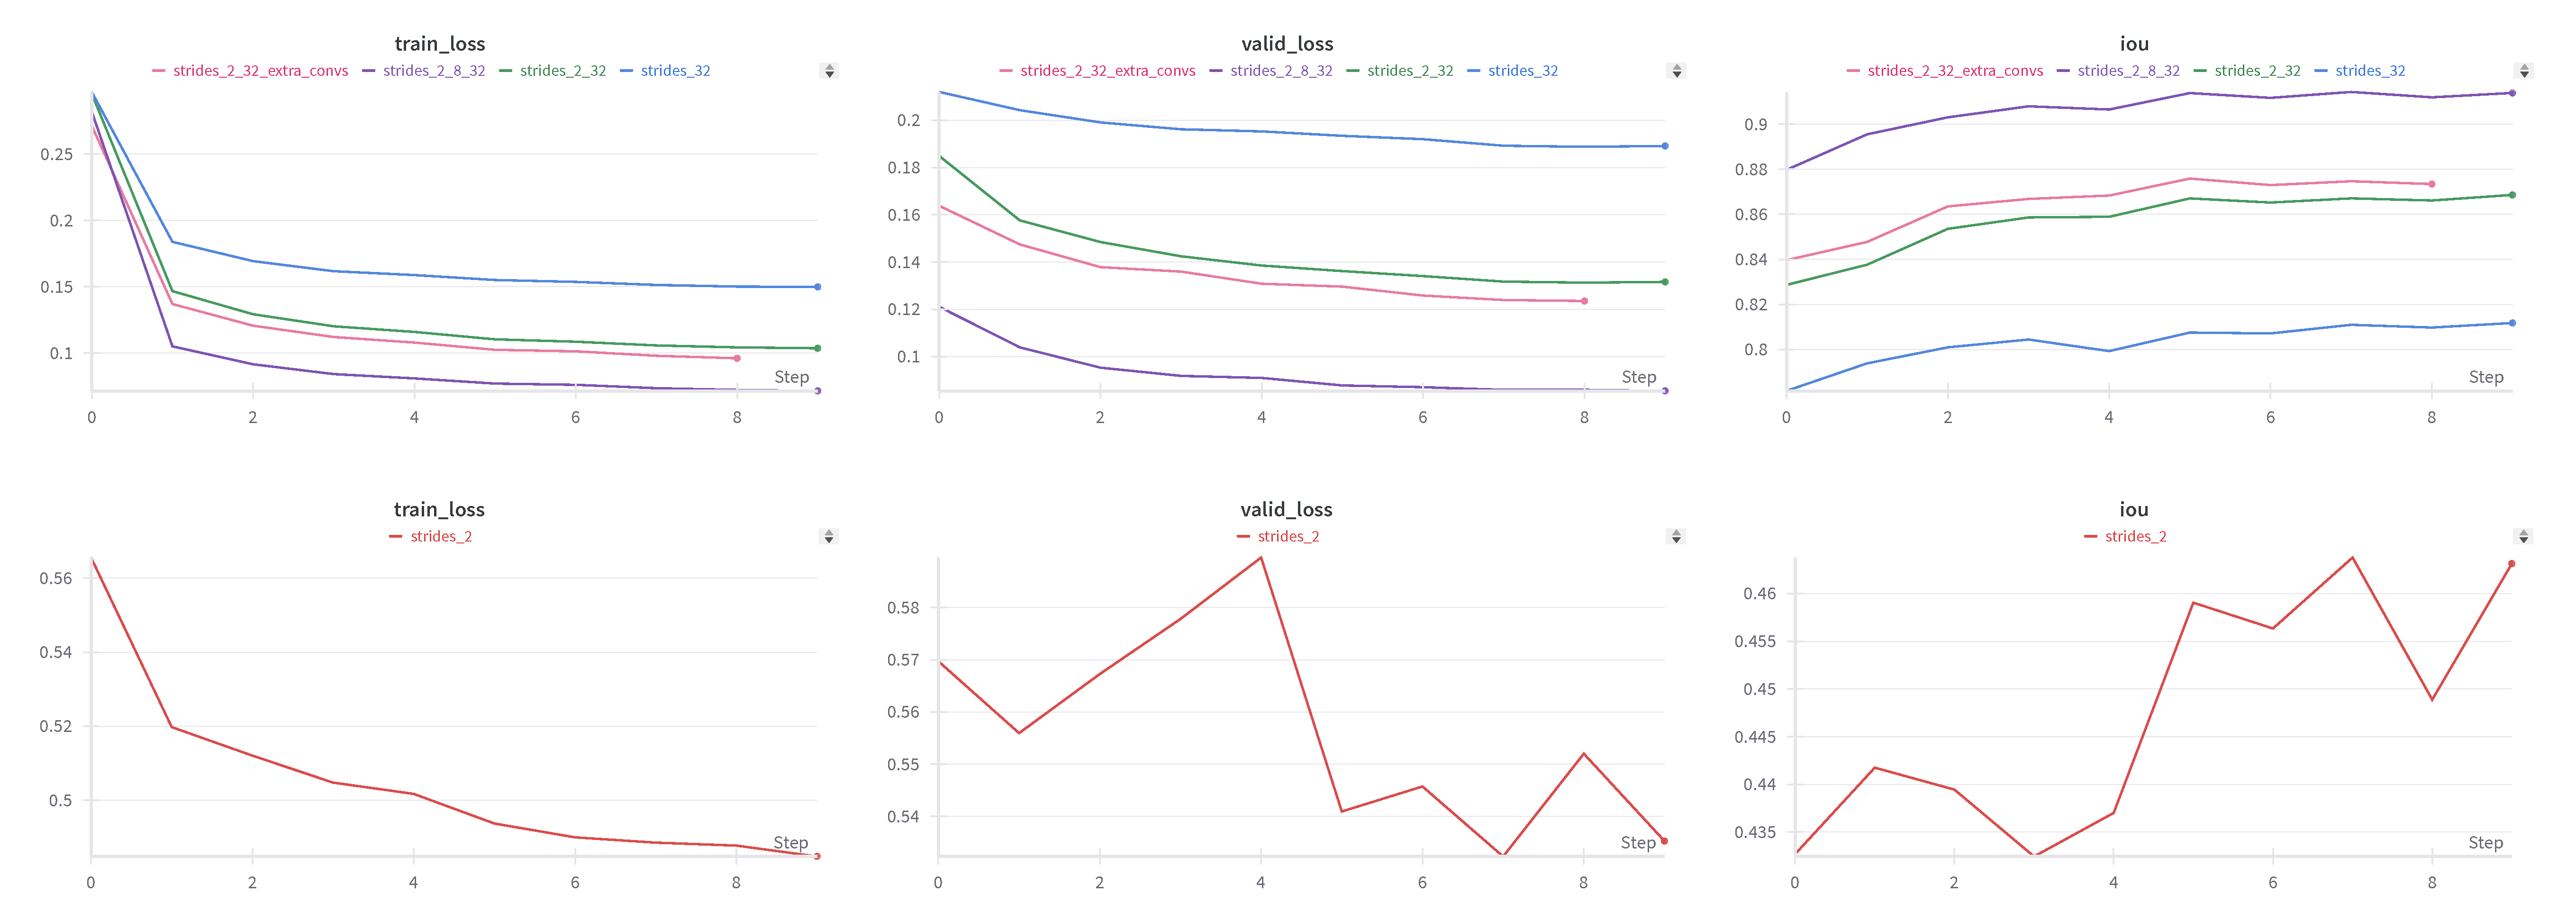
\includegraphics[width=0.98\textwidth]{imgs/training_metrics.pdf}
    \caption{Evolução das métricas de treinamento e validação ao longo das épocas.}
\end{figure*}


Entre eles, o modelo strides\_2\_8\_32 se destaca por atingir os menores valores de perda e os maiores valores de IoU, evidenciando uma aprendizagem mais eficiente, dado que este modelo possui a combinação de mapas de ativação de diferentes resoluções. 

Por outro lado, o modelo strides\_2 apresenta uma curva de \textit{train\_loss} elevada e instável, sugerindo dificuldade de aprendizado com apenas 10 épocas. No entanto, a curva de IoU apresenta uma tendência de subida, indicando que o modelo poderia melhorar com mais épocas de treinamento. 

Em síntese, as métricas de treinamento demonstram que a combinação de múltiplos strides resulta em aprendizado mais eficaz e estável, enquanto o uso isolado de stride 2 se mostra inadequado para a tarefa de segmentação.

\subsection{Segmentações e Comparação Qualitativa}

A Figura~\ref{fig:segmentations} apresenta exemplos de segmentações geradas pelos diferentes modelos avaliados. Cada linha corresponde a uma configuração do decodificador, permitindo observar as diferenças qualitativas nas máscaras de segmentação produzidas. É notório que os modelos com múltiplos strides (como strides\_2\_8\_32 e strides\_2\_32) conseguem capturar melhor os detalhes dos objetos segmentados, resultando em máscaras mais precisas e com menos artefatos. Enquanto o modelo strides\_2 apresenta segmentações mais imprecisas, com falhas significativas na delimitação dos objetos, indicando confusão entre o fundo e o objeto segmentado. Já o modelo strides\_32, apesar de ser capaz de segmentar os objetos, apresenta uma resolução mais baixa, resultando em máscaras menos detalhadas.


\begin{figure*}[htb]
    \centering
    \label{fig:segmentations}  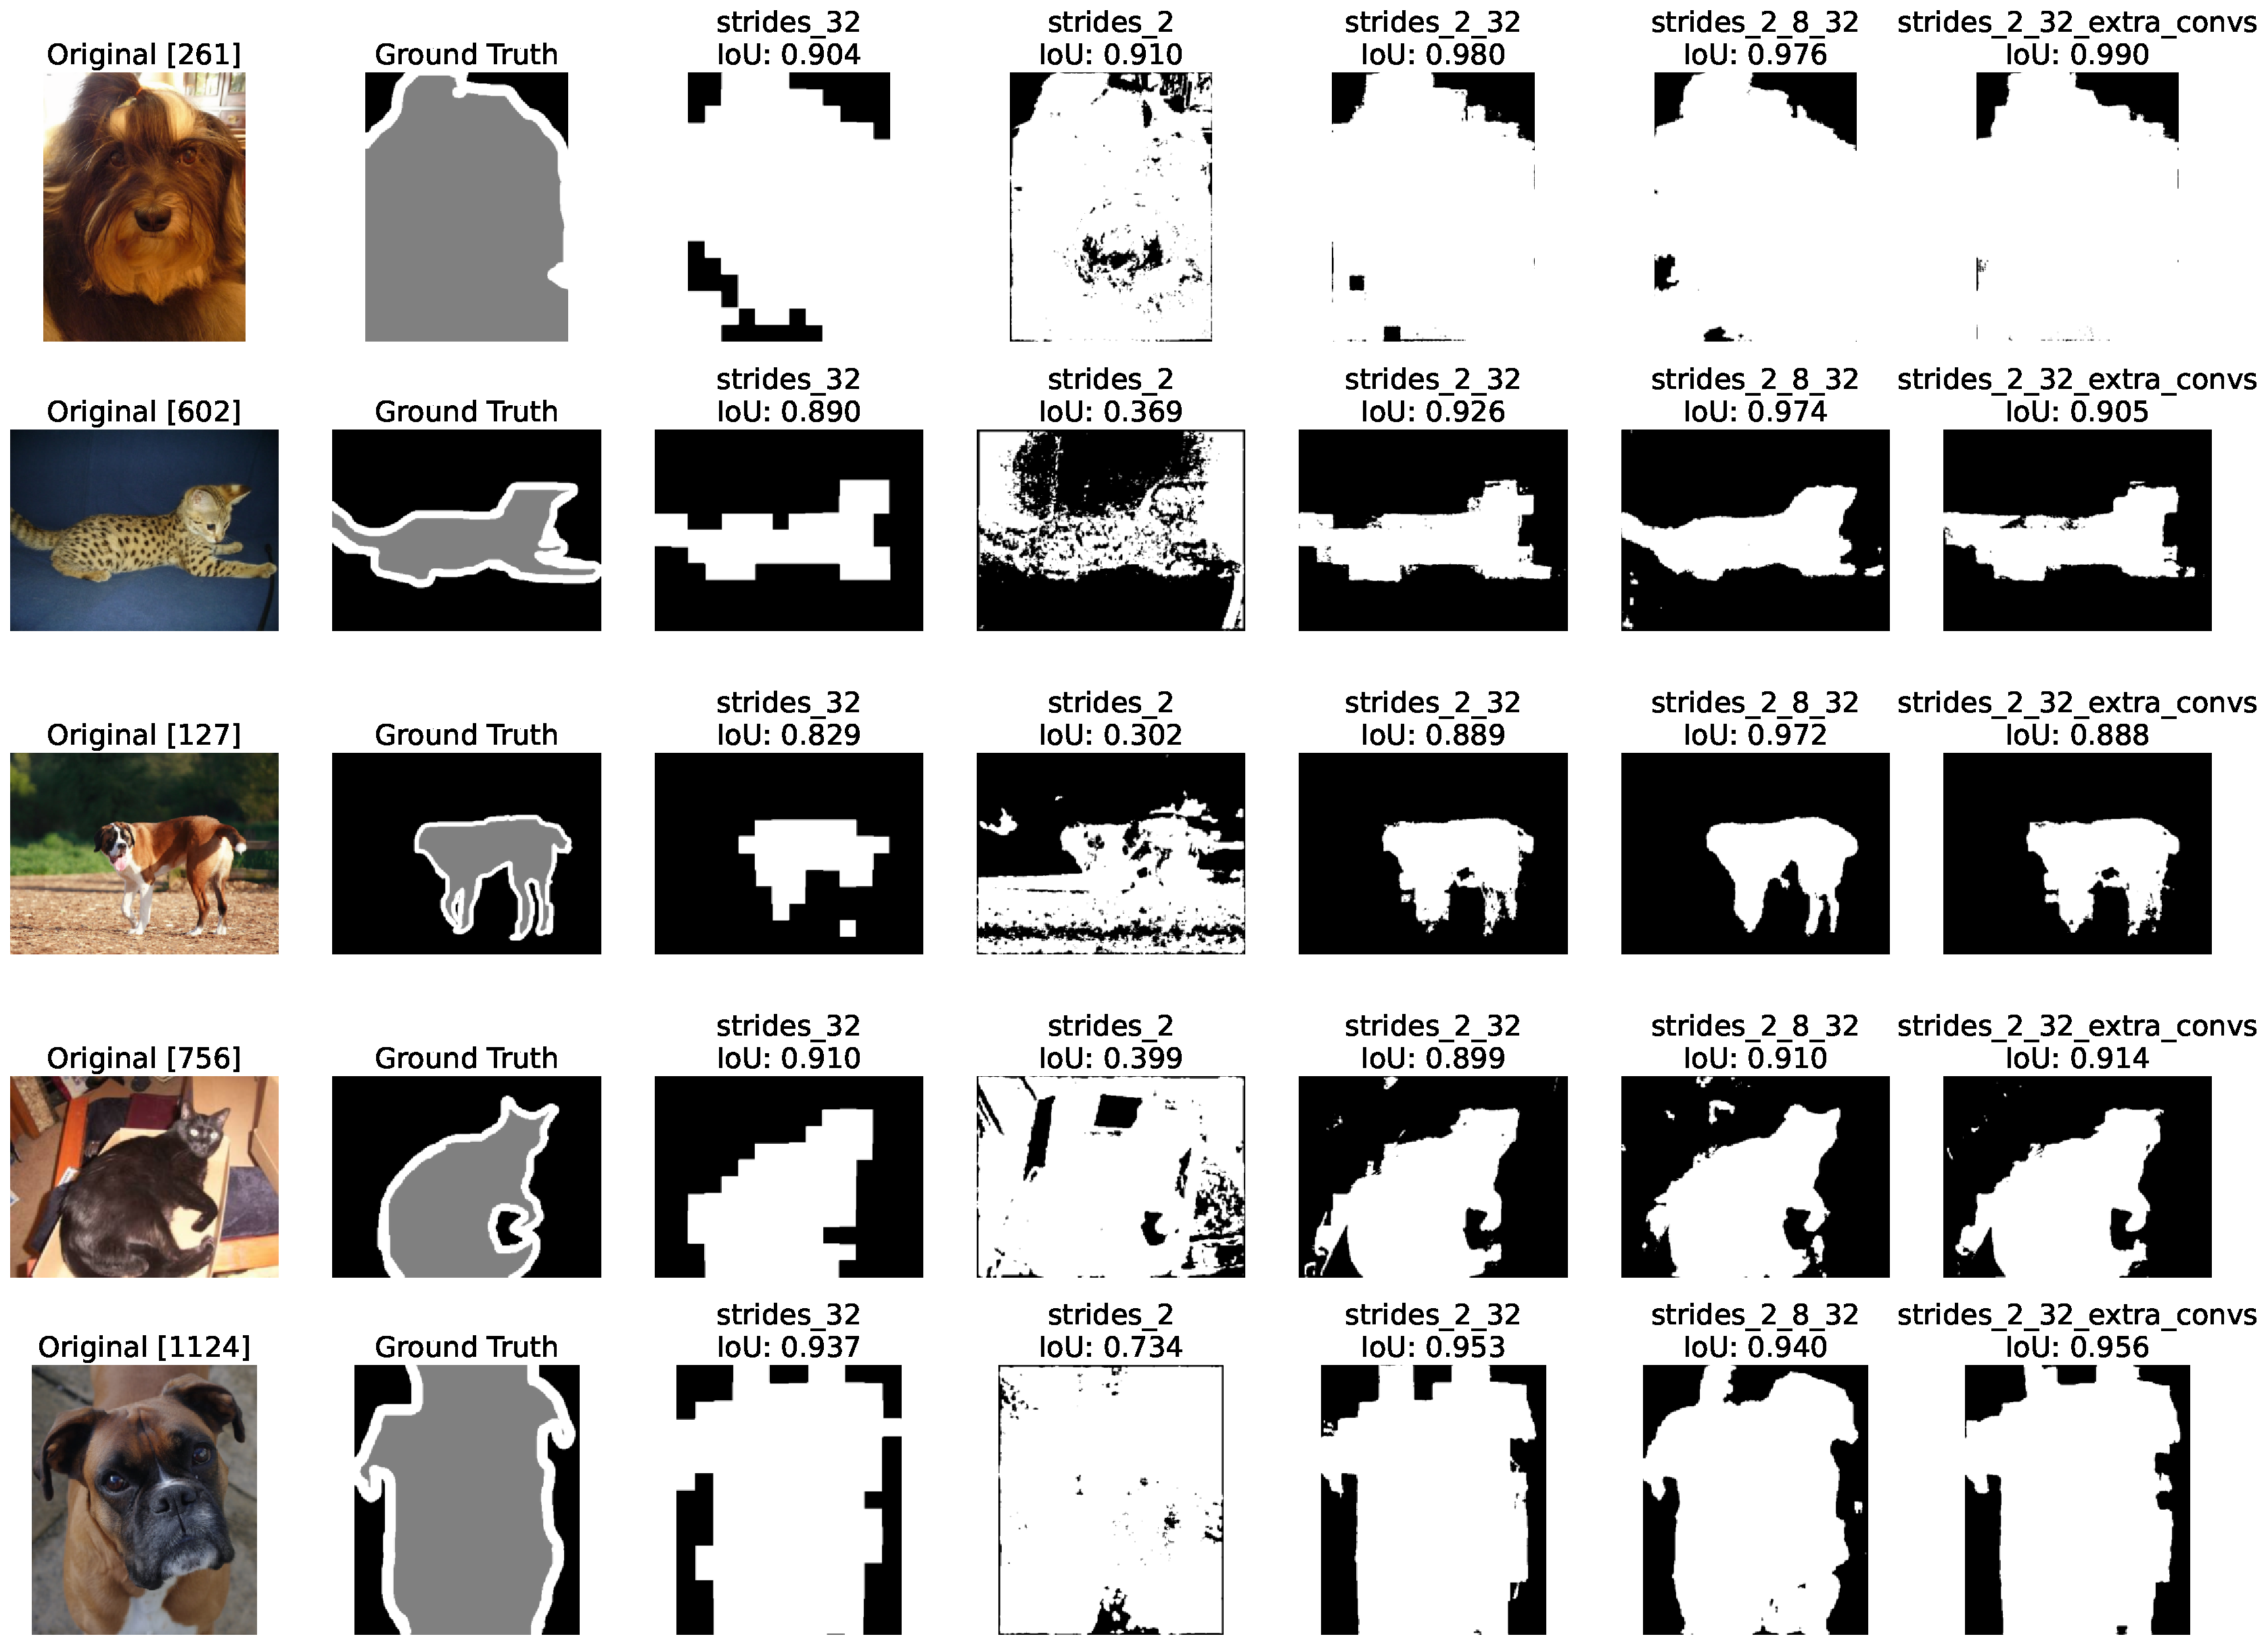
\includegraphics[width=0.98\textwidth]{imgs/segmentations.pdf}
    \caption{Exemplo de segmentações geradas pelos diferentes modelos. Cada linha representa uma configuração do decodificador.}
\end{figure*}



\subsection{Análise do Desempenho Quantitativo}
A Tabela~\ref{tab:performance} apresenta uma comparação direta dos modelos em métricas-chave de segmentação. O modelo strides\_2\_8\_32 destaca-se como o mais preciso, atingindo IoU médio de 0.729. Os modelos strides\_2\_32\_extra\_convs e strides\_2\_32 apresentam desempenho semelhante, com valores próximos a 0.706 e 0.701, respectivamente. O modelo strides\_32, embora funcional, apresenta resultado inferior (0.677), enquanto strides\_2 demonstra desempenho insatisfatório e alta variabilidade (IoU médio de 0.407, desvio padrão 0.200), evidenciando instabilidade.

\begin{table*}[b]
\caption{\label{tab:performance}
Desempenho dos modelos de decodificador nas métricas de segmentação.}
\begin{ruledtabular}
\begin{tabular}{lccc}
\hline
Modelo & IoU médio $\pm$ std & Parâmetros & Tempo total de inferência (s) \\
\hline
strides\_32              & 0.677 $\pm$ 0.130 & $2.674 \times 10^{7}$ & 13.928 \\
strides\_2               & 0.407 $\pm$ 0.200 & $2.560 \times 10^{7}$ & 14.073 \\
strides\_2\_32           & 0.701 $\pm$ 0.128 & $2.678 \times 10^{7}$ & 14.234 \\
strides\_2\_8\_32        & 0.729 $\pm$ 0.122 & $2.685 \times 10^{7}$ & 14.777 \\
strides\_2\_32\_extra\_convs & 0.706 $\pm$ 0.128 & $2.682 \times 10^{7}$ & 14.752 \\
\hline
\end{tabular}
\end{ruledtabular}
\end{table*}

Em relação à eficiência, todos os modelos de melhor desempenho possuem número de parâmetros semelhante, em torno de 26.7 a 26.8 milhões, e o tempo de inferência é praticamente constante entre eles. O modelo strides\_2\_8\_32 oferece o melhor equilíbrio entre precisão e custo computacional, já que o pequeno acréscimo no tempo de inferência é compensado pelo ganho em desempenho.

\section{Discussão}

Os resultados indicam que a inclusão de múltiplos strides no decodificador melhora a qualidade da segmentação, especialmente ao combinar strides baixos (maior resolução) com altos (maior contexto). O uso de camadas extras proporciona ganhos marginais, mas aumenta o custo computacional. O modelo com strides 2, 8 e 32 apresentou o melhor IoU médio, evidenciando que a combinação de diferentes escalas é benéfica para capturar detalhes e contexto.

O tempo de inferência permaneceu similar entre os modelos, com pequenas variações atribuídas ao número de parâmetros. Todos os modelos utilizaram encoder pré-treinado, o que acelerou o treinamento e permitiu boa generalização mesmo com poucas épocas.

\section{Conclusão}
O estudo realizado demonstra que a variação dos hiperparâmetros do decodificador impacta significativamente a qualidade da segmentação. Recomenda-se a combinação de múltiplos strides para cenários nos quais detalhes e contexto são importantes. O uso de camadas extras pode ser explorado para ganhos adicionais, desde que o custo computacional seja aceitável. Como possibilidade futura, sugere-se investigar decodificadores mais profundos, atenção espacial e integração com arquiteturas modernas como U-Net e DeepLab.


\bibliography{apssamp}

\end{document}